%%%%%%%%%%%%%%%%%%%%%%%%%%%%%%%%%%%%%%%%%
% Beamer Presentation
% LaTeX Template
% Version 1.0 (10/11/12)
%
% This template has been downloaded from:
% http://www.LaTeXTemplates.com
%
% License:
% CC BY-NC-SA 3.0 (http://creativecommons.org/licenses/by-nc-sa/3.0/)
%
%%%%%%%%%%%%%%%%%%%%%%%%%%%%%%%%%%%%%%%%%

%----------------------------------------------------------------------------------------
%	PACKAGES AND THEMES
%----------------------------------------------------------------------------------------

\documentclass[handout]{beamer}

\mode<presentation> {

% The Beamer class comes with a number of default slide themes
% which change the colors and layouts of slides. Below this is a list
% of all the themes, uncomment each in turn to see what they look like.

%\usetheme{default}
%\usetheme{AnnArbor}
%\usetheme{Antibes}
%\usetheme{Bergen}
%\usetheme{Berkeley}
%\usetheme{Berlin}
%\usetheme{Boadilla}
%\usetheme{CambridgeUS}
%\usetheme{Copenhagen}
%\usetheme{Darmstadt}
%\usetheme{Dresden}
%\usetheme{Frankfurt}
%\usetheme{Goettingen}
%\usetheme{Hannover}
%\usetheme{Ilmenau}
%\usetheme{JuanLesPins}
%\usetheme{Luebeck}
\usetheme{Madrid}
%\usetheme{Malmoe}
%\usetheme{Marburg}
%\usetheme{Montpellier}
%\usetheme{PaloAlto}
%\usetheme{Pittsburgh}
%\usetheme{Rochester}
%\usetheme{Singapore}
%\usetheme{Szeged}
%\usetheme{Warsaw}

% As well as themes, the Beamer class has a number of color themes
% for any slide theme. Uncomment each of these in turn to see how it
% changes the colors of your current slide theme.

%\usecolortheme{albatross}
%\usecolortheme{beaver}
%\usecolortheme{beetle}
%\usecolortheme{crane}
%\usecolortheme{dolphin}
%\usecolortheme{dove}
%\usecolortheme{fly}
%\usecolortheme{lily}
%\usecolortheme{orchid}
%\usecolortheme{rose}
%\usecolortheme{seagull}
%\usecolortheme{seahorse}
%\usecolortheme{whale}
%\usecolortheme{wolverine}

%\setbeamertemplate{footline} % To remove the footer line in all slides uncomment this line
%\setbeamertemplate{footline}[page number] % To replace the footer line in all slides with a simple slide count uncomment this line

%\setbeamertemplate{navigation symbols}{} % To remove the navigation symbols from the bottom of all slides uncomment this line
}

\usepackage{graphicx} % Allows including images
\usepackage{booktabs} % Allows the use of \toprule, \midrule and \bottomrule in tables
\usepackage{cool}
\usepackage{amsmath}
\usepackage{amssymb}
\usepackage{pseudocode}
\usepackage{bm}
\usepackage{multirow}
\usepackage{physics}
\usepackage{hyperref}
\usepackage{listings}
\usepackage{enumerate}
\usepackage{pifont}% http://ctan.org/pkg/pifont
\newcommand{\cmark}{\ding{51}}%
\newcommand{\xmark}{\ding{55}}%

\newcommand{\prob}{\mathcal{P}}
\newcommand{\rew}{\mathcal{R}}
\newcommand{\states}{\mathcal{S}}
\newcommand{\actions}{\mathcal{S}}

\DeclareMathOperator*{\argmin}{arg\,min}
\DeclareMathOperator*{\argmax}{arg\,max}

\newcommand{\vw}{\bm{V_w}}
\newcommand{\vpi}{\bm{V}^{\pi}}
\newcommand{\bphi}{\bm{\Phi}}
\newcommand{\bb}{\bm{B}^{\pi}}
\newcommand{\bpi}{\bm{\Pi_{\Phi}}}
\newcommand{\bmu}{\bm{\mu_{\pi}}}
\newcommand{\bv}{\bm{V}}
\newcommand{\bd}{\bm{D}}
\newcommand{\bw}{\bm{w}}
\newcommand{\btheta}{\bm{\theta}}
\newcommand{\bdel}{\bm{\delta_w}}
\newcommand{\brew}{\bm{\mathcal{R}}^{\pi}}
\newcommand{\bprob}{\bm{\mathcal{P}}^{\pi}}


%----------------------------------------------------------------------------------------
%	TITLE PAGE
%----------------------------------------------------------------------------------------

\title[Batch RL Chapter]{A Guided Tour of \href{http://stanford.edu/~ashlearn/RLForFinanceBook/book.pdf}{\underline{\textcolor{yellow}{Chapter 13}}}: \\ Batch RL, Experience-Replay, DQN, LSPI, Gradient TD} % The short title appears at the bottom of every slide, the full title is only on the title page

\author{Ashwin Rao} % Your name
\institute[Stanford] % Your institution as it will appear on the bottom of every slide, may be shorthand to save space
{ICME, Stanford University
 % Your institution for the title page
}

\date % Date, can be changed to a custom date

\begin{document}
\lstset{language=Python}  
\begin{frame}
\titlepage % Print the title page as the first slide
\end{frame}

% \begin{frame}
% \frametitle{Overview} % Table of contents slide, comment this block out to remove it
% \tableofcontents % Throughout your presentation, if you choose to use \section{} and \subsection{} commands, these will automatically be printed on this slide as an overview of your presentation
% \end{frame}

\begin{frame}
\frametitle{Moving on to practically sophisticated algorithms}
\begin{itemize}[<+->]
\item Let's examine the core pattern of RL Algorithms we've learnt so far
\item Experiences arrive one at a time, is used (for learning) and {\em discarded}
\item Learning is {\em incremental}, with VF update after each unit of experience
\item Are there alternative patterns we can employ? The answer is {\em Yes}
\item We highlight 2 key patterns that yield a richer range of RL Algorithms
\begin{enumerate}[<+->]
\item {\em Experience-Replay}: Store the data as it arrives, and re-use it
\item {\em Batch RL}: Learn the VF for an entire batch of data directly
\end{enumerate} 
\item Experience-Replay and Batch RL can be combined in interesting ways
\end{itemize}
\end{frame}



\begin{frame}
\frametitle{Incremental RL makes inefficient use of training data}
\begin{itemize}[<+->]
\item Incremental versus Batch RL in the context of fixed finite data
\item Let's understand the difference for the simple case of MC Prediction
\item Given fixed finite sequence of trace experiences yielding training data:
$$\mathcal{D} = [(S_i, G_i) | 1 \leq i \leq n]$$
\item Incremental MC estimates $V(s;\bm{w})$ using $\nabla_{\bm{w}} \mathcal{L}(\bm{w})$ for each data pair:
$$\mathcal{L}_{(S_i, G_i)}(\bm{w}) = \frac 1 2 \cdot (V(S_i; \bm{w}) - G_i)^2$$
$$\nabla_{\bm{w}} \mathcal{L}_{(S_i, G_i)}(\bm{w}) = (V(S_i; \bm{w}) - G_i) \cdot \nabla_{\bm{w}} V(S_i; \bm{w})$$
$$\Delta \bm{w} = \alpha \cdot (G_i - V(S_i; \bm{w})) \cdot \nabla_{\bm{w}} V(S_i; \bm{w})$$
\item $n$ updates are performed in sequence for $i = 1, 2, \ldots ,n$
\item Uses  \lstinline{update} method of \lstinline{FunctionApprox} for each data pair $(S_i, G_i)$
\item Incremental RL makes inefficient use of available training data $\mathcal{D}$
\item Essentially each data point is ``discarded'' after being used for update
\end{itemize}
\end{frame}


\begin{frame}
\frametitle{Batch MC Prediction makes efficient use of training data}
\pause
\begin{itemize}[<+->]
\item Instead we'd like to estimate the Value Function $V(s;\bm{w^*})$ such that
\begin{align*}
\bm{w^*} & = \argmin_{\bm{w}} \frac 1 n \cdot \sum_{i=1}^n \frac 1 2 \cdot (V(S_i;\bm{w}) - G_i)^2 \\
& = \argmin_{\bm{w}} \mathbb{E}_{(S,G) \sim \mathcal{D}} [\frac 1 2 \cdot (V(S; \bm{w}) - G)^2]
\end{align*}
\item This is the \lstinline{solve} method of \lstinline{FunctionApprox} on training data $\mathcal{D}$
\item This approach to RL is known as {\em Batch RL}
\item \lstinline{solve} by doing \lstinline{update}s with repeated use of available data pairs
\item Each update using random data pair $(S,G) \sim \mathcal{D}$
$$\Delta \bm{w} = \alpha \cdot (G - V(S; \bm{w})) \cdot \nabla_{\bm{w}} V(S; \bm{w})$$
\item This will ultimately converge to desired value function $V(s;\bm{w^*})$
\item Repeated use of available data  known as {\em Experience-Replay} 
\item This makes more efficient use of available training data $\mathcal{D}$
\end{itemize}
\end{frame}

\begin{frame}
\frametitle{Batch TD Prediction makes efficient use of Experiences}
\pause
\begin{itemize}[<+->]
\item In Batch TD Prediction, we have experiences data $\mathcal{D}$ available as:
$$\mathcal{D} = [(S_i, R_i, S'_i) | 1 \leq i \leq n]$$
\item Where $(R_i, S'_i)$ is the pair of reward and next state from a state $S_i$
\item So, Experiences $\mathcal{D}$ in the form of finite number of atomic experiences
\item This is represented in code as an \lstinline{Iterable[TransitionStep[S]]}
\item Parameters updated with repeated use of these atomic experiences
\item Each update using random data pair $(S,R,S') \sim \mathcal{D}$
$$\Delta \bm{w} = \alpha \cdot (R + \gamma \cdot V(S'; \bm{w}) - V(S; \bm{w})) \cdot \nabla_{\bm{w}} V(S; \bm{w})$$
\item This is TD Prediction with Experience-Replay on Finite Experiences $\mathcal{D}$
\end{itemize}
\end{frame}

\begin{frame}
\frametitle{Batch TD($\lambda$) Prediction}
\pause
\begin{itemize}[<+->]
\item In Batch TD($\lambda$) Prediction, given finite number of trace experiences
$$\mathcal{D} = [(S_{i,0}, R_{i,1}, S_{i,1}, R_{i,2}, S_{i,2}, \ldots, R_{i,T_i}, S_{i,T_i}) | 1 \leq i \leq n]$$
\item Parameters updated with repeated use of these trace experiences
\item Randomly pick trace experience (say indexed $i$) $\sim \mathcal{D}$
\item For trace experience $i$, parameters updated at each time step $t$:
$$\bm{E}_t = \gamma \lambda \cdot \bm{E}_{t-1} + \nabla_{\bm{w}} V(S_{i,t};\bm{w})$$
$$\Delta \bm{w} = \alpha \cdot (R_{i,t+1} + \gamma \cdot V(S_{i,t+1}; \bm{w}) - V(S_{i,t}; \bm{w})) \cdot \bm{E}_t$$
\end{itemize}
\end{frame}

\begin{frame}
\frametitle{The Deep Q-Networks (DQN) Control Algorithm}
\pause
DQN uses {\bf Experience-Replay} and {\bf fixed Q-learning targets}.\\
\pause
At each time $t$ for each episode:
\begin{itemize}[<+->]
\item Given state $S_t$, take action $A_t$ according to $\epsilon$-greedy policy extracted from Q-network values $Q(S_t,a;\bm{w})$
\item Given state $S_t$ and action $A_t$, obtain reward $R_{t+1}$ and next state $S_{t+1}$
\item Store atomic experience $(S_t, A_t, R_{t+1}, S_{t+1})$ in replay memory $\mathcal{D}$
\item Sample random mini-batch  of atomic experiences $(s_i,a_i,r_i,s'_i) \sim \mathcal{D}$
\item Update Q-network parameters $\bm{w}$ using Q-learning targets based on ``frozen'' parameters $\bm{w}^-$ of {\em target network}
$$\Delta \bm{w} = \alpha \cdot \sum_i (r_i + \gamma \cdot \max_{a'_i} Q(s'_i, a'_i; \bm{w}^-) - Q(s_i,a_i;\bm{w})) \cdot \nabla_{\bm{w}} Q(s_i,a_i;\bm{w})$$ 
\item $S_t \leftarrow S_{t+1}$
\end{itemize}
\pause
Parameters $\bm{w}^-$ of target network infrequently updated to values of Q-network parameters $\bm{w}$ (hence, Q-learning targets treated as ``frozen'')
\end{frame}

\begin{frame}
\frametitle{Least-Squares RL Prediction}
\pause
\begin{itemize}[<+->]
\item Batch RL Prediction for general function approximation is iterative
\item Uses Experience-Replay and Gradient Descent
\item We can solve directly (without gradient) for linear function approx
\item Define a sequence of feature functions $\phi_j: \mathcal{S} \rightarrow \mathbb{R}, j = 1, 2, \ldots, m$
\item Parameters $w$ is a weights vector $\bm{w} = (w_1, w_2, \ldots, w_m) \in \mathbb{R}^m$
\item Value Function is approximated as:
$$V(s;\bm{w}) = \sum_{j=1}^m \phi_j(s) \cdot w_j = \bm{\phi}(s)^T \cdot \bm{w}$$
where $\bm{\phi}(s) \in \mathbb{R}^m$ is the feature vector for state $s$
\end{itemize}
\end{frame}


\begin{frame}
\frametitle{Least-Squares Monte-Carlo (LSMC)}
\pause
\begin{itemize}[<+->]
\item Loss function for Batch MC Prediction with data $[(S_i, G_i) | 1 \leq i \leq n]$:
$$\mathcal{L}(\bm{w}) =  \frac 1 {2n} \cdot \sum_{i=1}^n (\sum_{j=1}^m \phi_j(S_i) \cdot w_j - G_i)^2 = \frac 1 {2n} \cdot \sum_{i=1}^n (\bm{\phi}(S_i)^T \cdot \bm{w} - G_i)^2$$
\item The gradient of this Loss function is set to 0 to solve for $\bm{w}^*$
$$\sum_{i=1}^n \bm{\phi}(S_i) \cdot (\bm{\phi}(S_i)^T \cdot \bm{w^*} - G_i) = 0$$
\item $\bm{w^}*$ is solved as $\bm{A}^{-1} \cdot \bm{b}$
\item $m \times m$ Matrix $\bm{A}$ is accumulated at each data pair $(S_i, G_i)$ as:
$$ \bm{A} \leftarrow \bm{A} + \bm{\phi}(S_i) \cdot \bm{\phi}(S_i)^T \text{ (i.e., outer-product of } \bm{\phi}(S_i) \text{ with itself})$$
\item $m$-Vector $\bm{b}$ is accumulated at each data pair $(S_i, G_i)$ as:
$$\bm{b} \leftarrow \bm{b} + \bm{\phi}(S_i) \cdot G_i$$
\item Sherman-Morrison incremental inverse can be done in $O(m^2)$
\end{itemize}
\end{frame}

\begin{frame}
\frametitle{Least-Squares Temporal-Difference (LSTD)}
\pause
\begin{itemize}[<+->]
\item Loss func for Batch TD Prediction with data $[(S_i, R_i, S'_i) | 1 \leq i \leq n]$:
$$\mathcal{L}(\bm{w}) = \frac 1 {2n} \cdot \sum_{i=1}^n (\bm{\phi}(S_i)^T \cdot \bm{w} - (R_i + \gamma \cdot \bm{\phi}(S'_i)^T \cdot \bm{w}))^2$$
\item The semi-gradient of this Loss function is set to 0 to solve for $\bm{w}^*$
$$\sum_{i=1}^n \bm{\phi}(S_i) \cdot (\bm{\phi}(S_i)^T \cdot \bm{w^*} - (R_i + \gamma \cdot \bm{\phi}(S'_i)^T \cdot \bm{w}^*)) = 0$$
\item $\bm{w}^*$ is solved as $\bm{A}^{-1} \cdot \bm{b}$
\item $m \times m$ Matrix $\bm{A}$ is accumulated at each atomic experience $(S_i, R_i, S'_i)$:
$$ \bm{A} \leftarrow \bm{A} + \bm{\phi}(S_i) \cdot (\bm{\phi}(S_i) - \gamma \cdot \bm{\phi}(S'_i))^T \text{ (note the Outer-Product)}$$
\item $m$-Vector $\bm{b}$ is accumulated at each atomic experience $(S_i, R_i, S'_i)$:
$$\bm{b} \leftarrow \bm{b} + \bm{\phi}(S_i) \cdot R_i$$
\item Sherman-Morrison incremental inverse can be done in $O(m^2)$
\end{itemize}
\end{frame}

\begin{frame}
\frametitle{LSTD($\lambda$)}
\pause
\begin{itemize}[<+->]
\item Likewise, we can do LSTD($\lambda$) using Eligibility Traces
\item Denote the Eligibility Traces of atomic experience $i$ as $\bm{E}_i$
\item Note: $\bm{E}_i$ accumulates $\nabla_{\bm{w}} V(s;\bm{w}) = \bm{\phi}(s)$ in each trace experience
\item When accumulating, previous step's eligibility traces discounted by $\lambda \gamma$
$$\sum_{i=1}^n \bm{E_i} \cdot (\bm{\phi}(S_i)^T \cdot \bm{w^*} - (R_i + \gamma \cdot \bm{\phi}(S'_i)^T \cdot \bm{w}^*)) = 0$$
\item $\bm{w}^*$ is solved as $\bm{A}^{-1} \cdot \bm{b}$
\item $m \times m$ Matrix $\bm{A}$ is accumulated at each atomic experience $(S_i, R_i, S'_i)$:
$$ \bm{A} \leftarrow \bm{A} + \bm{E_i} \cdot (\bm{\phi}(S_i) - \gamma \cdot \bm{\phi}(S'_i))^T \text{ (note the Outer-Product)}$$
\item $m$-Vector $\bm{b}$ is accumulated at each atomic experience $(S_i, R_i, S'_i)$ as:
$$\bm{b} \leftarrow \bm{b} + \bm{E_i} \cdot R_i$$
\item Sherman-Morrison incremental inverse can be done in $O(m^2)$
\end{itemize}
\end{frame}

\begin{frame}
\frametitle{Convergence of Least Squares Prediction Algorithms}
\pause
\begin{center}
      \begin{tabular}{ccccc}
      \hline
      On/Off Policy & Algorithm & Tabular & Linear & Non-Linear \\ \hline
      \multirow{3}{*}{On-Policy} & MC & \cmark & \cmark & \cmark \\
      & {\bf LSMC} & \cmark & \cmark & - \\
      & TD & \cmark & \cmark & \xmark \\ 
      & {\bf LSTD} & \cmark & \cmark & - \\ \hline
      \multirow{3}{*}{Off-Policy} & MC & \cmark & \cmark & \cmark \\
      & {\bf LSMC} & \cmark & \xmark & - \\
      & TD & \cmark & \xmark & \xmark \\
      & {\bf LSTD} & \cmark & \xmark & - \\ \hline
      \end{tabular}
\end{center}      
\end{frame}

\begin{frame}
\frametitle{Least Squares RL Control}
\pause
\begin{itemize}[<+->]
\item To perform Least Squares RL Control, we do GPI with:
\begin{itemize}[<+->]
\item Policy Evaluation as Least-Squares Q-Value Prediction
\item Greedy (or $\epsilon$-Greedy) Policy Improvement
\end{itemize}
\item For On-Policy MC/TD Control, Q-Value Prediction (for policy $\pi$):
$$Q^{\pi}(s,a) \approx Q(s,a;\bm{w}^*) = \bm{\phi}(s,a)^T \cdot \bm{w}^*$$
\item Direct solve for $\bm{w}^*$ using experiences data generated using policy $\pi$
\item We are interested in Off-Policy Control with Least-Squares TD
\item Using the same idea as Q-Learning and with Experience-Replay
\item This technique is known as Least Squares Policy Iteration (LSPI)
\end{itemize}
\end{frame}

\begin{frame}
\frametitle{Least Squares Policy Iteration (LSPI)}
\pause
\begin{itemize}[<+->]
\item Input is fixed finite data set $\mathcal{D}$ consisting of $(s,a,r,s')$ experiences
\item Goal is to determine Optimal Q-Value Linear Function Approximation
\item Each iteration of GPI starts with a deterministic target policy $\pi_D$
\item $\pi_D$ is made available from the previous iteration of GPI
\item Goal of the iteration is to solve for weights $\bm{w}^*$ to minimize:
\begin{align*}
\mathcal{L}(\bm{w}) & = \sum_i (Q(s_i,a_i; \bm{w}) - (r_i + \gamma \cdot Q(s'_i,\pi_D(s'_i); \bm{w})))^2\\
& = \sum_i (\bm{\phi}(s_i,a_i)^T \cdot \bm{w} - (r_i + \gamma \cdot \bm{\phi}(s'_i, \pi_D(s'_i))^T \cdot \bm{w}))^2
\end{align*}
\item Solved using sampled mini-batch of experiences $(s_i,a_i,r_i,s'_i)$ from $\mathcal{D}$
\item This solved $\bm{w}^*$ defines an updated Q-Value Function
\item Iteration ends by setting the target policy $\pi_D$ (for next iteration) as:
$$\pi_D(s) = \argmax_a Q(s,a; \bm{w}^*)$$
\end{itemize}
\end{frame}

\begin{frame}
\frametitle{Solving for weights $\bm{w}^*$ with LSTDQ}
\pause
\begin{itemize}[<+->]
\item We set the semi-gradient of $\mathcal{L}(\bm{w})$ at $\bm{w} = \bm{w}^*$ to 0
\begin{equation}
\sum_i \phi(s_i,a_i) \cdot (\bm{\phi}(s_i,a_i)^T \cdot \bm{w}^* - (r_i + \gamma \cdot \bm{\phi}(s'_i, \pi_D(s'_i))^T \cdot \bm{w}^*)) = 0
\label{eq:lspi-loss-semi-gradient}
\end{equation}
\item $\bm{w}^*$ is solved as $\bm{A}^{-1} \cdot \bm{b}$
\item $m \times m$ Matrix $\bm{A}$ is accumulated at each experience $(s_i,a_i,r_i,s'_i)$:
$$ \bm{A} \leftarrow \bm{A} + \bm{\phi}(s_i, a_i) \cdot (\bm{\phi}(s_i, a_i) - \gamma \cdot \bm{\phi}(s'_i, \pi_D(s'_i)))^T $$
\item $m$-Vector $\bm{b}$ is accumulated at each experience $(s_i,a_i,r_i,s'_i)$ as:
$$\bm{b} \leftarrow \bm{b} + \bm{\phi}(s_i, a_i) \cdot r_i$$
\item Sherman-Morrison incremental inverse can be done in $O(m^2)$
\item This least-squares solution of $\bm{w}^*$ (Prediction) is known as {\em LSTDQ}
\item GPI with LSTDQ and greedy policy improvement known as {\em LSPI}
\end{itemize}
\end{frame}

\begin{frame}
\frametitle{Convergence of Control Algorithms}
\pause
\begin{center}
      \begin{tabular}{cccc}
      \hline
      Algorithm & Tabular & Linear & Non-Linear \\ \hline
      MC Control & \cmark & ( \cmark ) & \xmark \\
      SARSA & \cmark & ( \cmark ) & \xmark \\ 
      Q-Learning & \cmark & \xmark & \xmark \\
      {\bf LSPI} & \cmark & ( \cmark ) & - \\ \hline
      \end{tabular}
 \end{center}     
  \pause
  ( \cmark ) means it chatters around near-optimal Value Function   
\end{frame}


\begin{frame}
\frametitle{LSPI for Optimal Exercise of American Options}
\pause
\begin{itemize}[<+->]
\item American Option Pricing is Optimal Stopping, and hence an MDP
\item So can be tackled with Dynamic Programming or RL algorithms
\item But let us first review the mainstream approaches
\item For some American options, just price the European, eg: vanilla call
\item When payoff is not path-dependent and state dimension is not large, we can do backward induction on a binomial/trinomial tree/grid
\item Otherwise, the standard approach is \href{https://people.math.ethz.ch/~hjfurrer/teaching/LongstaffSchwartzAmericanOptionsLeastSquareMonteCarlo.pdf}{\underline{\textcolor{blue}{Longstaff-Schwartz algorithm}}}
\item Longstaff-Schwartz algorithm combines 3 ideas:
\begin{itemize}
\item Valuation based on Monte-Carlo simulation
\item Function approximation of continuation value for in-the-money states
\item Backward-recursive determination of early exercise states
\end{itemize}
\item We consider LSPI as an alternative approach for American Pricing
\end{itemize}
\end{frame}

\begin{frame}
\frametitle{LSPI as an alternative to Longstaff-Schwartz}
\pause
\begin{itemize}[<+->]
\item RL is straightforward if we clearly define the MDP
\item {\em State} is [Current Time, History of Underlying Security Prices]
\item {\em Action} is Boolean: Exercise (i.e., Stop) or Continue
\item {\em Reward} always 0, except upon Exercise ($=$ Payoff)
\item {\em State}-transitions based on Underlying Security's Risk-Neutral Process
\item Key is function approximation of state-conditioned continuation value
\item Continuation Value $\Rightarrow$ Optimal Stopping $\Rightarrow$ Option Price
\item We customize LSPI to Optimal Exercise of American Options
\item Based on \href{http://proceedings.mlr.press/v5/li09d/li09d.pdf}{\underline{\textcolor{blue}{this paper by Li, Szepesvari, Schuurmans}}}
\end{itemize}
\end{frame}

\begin{frame}
\frametitle{LSPI customized for American Options Pricing}
\pause
\begin{itemize}[<+->]
\item 2 actions: $a=c$ (continue the option) and $a=e$ (exercise the option)
\item Create function approx representation for $Q(s,a)$ only for $a=c$ since we know option payoff $g(s)$ for $a=e$, i.e., $Q(s,a) = g(s)$
$$
\hat{Q}(s,a; \bm{w}) =
\begin{cases}
\bm{\phi}(s)^T \cdot \bm{w} & \text{ if } a = c \\
g(s) & \text{ if } a = e
\end{cases}
$$
for feature funcs $\bm{\phi}(\cdot) = [\phi_i(\cdot)|i = 1, \ldots, m]$ of only state \& not action
\item Each iteration of GPI starts with a deterministic target policy $\pi_D$
\item $\pi_D$ is greedy policy from previous iteration's solved $Q(s,a;\bm{w}^*)$
\item Since we learn Q-Value function for only $a=c$, behavior policy $\mu$ generating experiences data for training is a constant func $\mu(s) = c$
\item Also, for American Options, the reward for $a=c$ is 0
\item So each atomic experiences for training is of the form $(s,c,0,s')$
\item So we represent each atomic experience for training as a 2-tuple $(s,s')$
\end{itemize}
\end{frame}

\begin{frame}
\frametitle{LSPI customized for American Options Pricing}
\pause
\begin{itemize}[<+->]
\item This reduces LSPI Semi-Gradient Equation \eqref{eq:lspi-loss-semi-gradient} to:
\begin{equation}
\sum_i \bm{\phi}(s_i) \cdot (\bm{\phi}(s_i)^T \cdot \bm{w}^* - \gamma \cdot \hat{Q}(s'_i, \pi_D(s'_i); \bm{w}^*)) = 0
\label{eq:customized-lspi-loss-semi-gradient}
\end{equation}
\item We need to consider two cases for the term $\hat{Q}(s'_i, \pi_D(s'_i); \bm{w}^*)$
\begin{itemize} 
\item  $C1$: If $s'_i$ is non-terminal and $\pi_D(s'_i) = c$ (i.e., $\bm{\phi}(s'_i)^T \cdot \bm{w} \geq g(s'_i)$):\\
Substitute $\bm{\phi}(s'_i)^T \cdot \bm{w}^*$ for $\hat{Q}(s'_i,\pi_D(s'_i); \bm{w}^*)$ in Equation \eqref{eq:customized-lspi-loss-semi-gradient}
\item $C2$: If $s'_i$ is a terminal state or $\pi_D(s'_i) = e$ (i.e., $g(s'_i) > \bm{\phi}(s'_i)^T \cdot \bm{w}$):\\
Substitute $g(s'_i)$ for $\hat{Q}(s'_i,\pi_D(s'_i); \bm{w}^*)$ in Equation \eqref{eq:customized-lspi-loss-semi-gradient}
\end{itemize}
\item So rewrite Equation \eqref{eq:customized-lspi-loss-semi-gradient} using indicator notation for cases $C1, C2$ as:
$$\sum_i \bm{\phi}(s_i) \cdot (\bm{\phi}(s_i)^T \cdot \bm{w}^* - \mathbb{I}_{C1} \cdot \gamma \cdot \bm{\phi}(s'_i)^T \cdot \bm{w}^*  -  \mathbb{I}_{C2} \cdot \gamma \cdot g(s'_i)) = 0$$
\item Factoring out $\bm{w}^*$, we get:
$$(\sum_i \bm{\phi}(s_i) \cdot (\bm{\phi}(s_i) - \mathbb{I}_{C1} \cdot \gamma \cdot \bm{\phi}(s'_i))^T) \cdot \bm{w}^*= \gamma \cdot \sum_i  \mathbb{I}_{C2} \cdot \bm{\phi}(s_i) \cdot g(s'_i)$$


\end{itemize}
\end{frame}

\begin{frame}
\frametitle{LSPI customized for American Options Pricing}
\pause
\begin{itemize}[<+->]
\item This can be written in the familiar vector-matrix notation: $\bm{A} \cdot \bm{w}^* = \bm{b}$
$$\bm{A} = \sum_i \bm{\phi}(s_i) \cdot (\bm{\phi}(s_i) - \mathbb{I}_{C1} \cdot \gamma \cdot \bm{\phi}(s'_i))^T$$
$$\bm{b} = \gamma \cdot \sum_i \mathbb{I}_{C2} \cdot \bm{\phi}(s_i) \cdot  g(s'_i)$$
\item $m \times m$ Matrix $\bm{A}$ is accumulated at each atomic experience $(s_i,s'_i)$ as:
$$\bm{A} \leftarrow \bm{A} + \bm{\phi}(s_i) \cdot (\bm{\phi}(s_i) -  \mathbb{I}_{C1} \cdot \gamma \cdot \bm{\phi}(s'_i))^T$$
\item $m$-Vector $\bm{b}$ is accumulated at each atomic experience $(s_i, s'_i)$ as:
$$\bm{b} \leftarrow \bm{b} + \gamma  \cdot \mathbb{I}_{C2} \cdot \bm{\phi}(s_i) \cdot g(s'_i)$$
\item Sherman-Morrison incremental inverse of $\bm{A}$ can be done in $O(m^2)$
\end{itemize}
\end{frame}


\begin{frame}
\frametitle{Feature functions}
\pause
\begin{itemize}[<+->]
\item Li, Szepesvari, Schuurmans recommend Laguerre polynomials (first 4)
\item Over $M_t = S_t/K$ where $S_t$ is underlying price and $K$ is strike
\item $\phi_0(S_t) = 1, \phi_1(S_t) = e^{-\frac {M_t} 2}, \phi_2(S_t) = e^{-\frac{M_t} 2} \cdot (1-M_t), \phi_3(S_t) = e^{-\frac{M_t} 2} \cdot (1-2M_t+M_t^2/2)$
\item They used these for Longstaff-Schwartz as well as for LSPI
\item For LSPI, we also need feature functions for time
\item They recommend $\phi_0^{(t)}(t) = sin(\frac {\pi(T-t)} {2T}), \phi_1^{(t)}(t) = \log(T-t), \phi_2^{(t)}(t) = (\frac t T)^2$
\end{itemize}
\end{frame}

\begin{frame}
\frametitle{Deep Q-Learning for American Pricing}
\pause
\begin{itemize}[<+->]
\item LSPI is data-efficient/compute-efficient, but linearity is a limitation
\item Alternative is (incremental) Q-Learning with neural network approx
\item We employ the same set up as LSPI (including Experience-Replay)
$$
\hat{Q}(s,a; \bm{w}) =
\begin{cases}
f(s;\bm{w}) & \text{ if } a = c \\
g(s) & \text{ if } a = e
\end{cases}
$$
where $f(s; \bm{w})$ is the deep neural network function approximation
\item Q-Learning update for each atomic experience $(s_i,s'_i)$
$$\Delta \bm{w} = \alpha \cdot (\gamma \cdot \hat{Q}(s'_i, \pi(s'_i); \bm{w}) - f(s_i;\bm{w})) \cdot \nabla_{\bm{w}} f(s_i;\bm{w})$$
\item When $s'_i$ is a non-terminal state, the update is:
$$\Delta \bm{w} =  \alpha \cdot (\gamma \cdot \max(g(s'_i), f(s'_i;\bm{w})) - f(s_i;\bm{w})) \cdot \nabla_{\bm{w}} f(s_i;\bm{w})$$
\item When $s'_i$ is a terminal state, the update is:
$$\Delta \bm{w} = \alpha \cdot (\gamma \cdot g(s'_i) - f(s_i;\bm{w})) \cdot \nabla_{\bm{w}} f(s_i;\bm{w})$$
\end{itemize}
\end{frame}

\begin{frame}
\frametitle{Motivation for understanding Value Function Geometry}
\pause
\begin{itemize}[<+->]
\item Helps us better understand transformations of Value Functions (VFs)
\item Across the various DP and RL algorithms
\item Particularly helps when VFs are approximated, esp. with linear approx
\item Provides insights into stability and convergence
\item Particularly when dealing with the ``Deadly Triad''
\item Deadly Triad := [Bootstrapping, Func Approx, Off-Policy]
\item {\bf Leads us to Gradient TD}
\end{itemize}
\end{frame}

\begin{frame}
\frametitle{Notation}
\pause
\begin{itemize}[<+->]
\item Assume finite state space $\mathcal{S} = \mathcal{N} = \{s_1, s_2, \ldots, s_n\}$
\item Action space $\mathcal{A}$ consisting of finite number of actions
\item This exposition can be extended to infinite/continuous spaces
\item This exposition is for a fixed (often stochastic) policy denoted $\pi(s,a)$
\item VF for a policy $\pi$ is denoted as $\vpi: \mathcal{S} \rightarrow \mathbb{R}$
\item $m$ feature functions $\phi_1, \phi_2, \ldots, \phi_m : \mathcal{S} \rightarrow \mathbb{R}$
\item Feature vector for a state $s \in \mathcal{S}$ denoted as $\bm{\phi}(s) \in \mathbb{R}^m$
\item For linear function approximation of VF with weights $\bw = (w_1, w_2, \ldots, w_m)$,
VF $\vw: \mathcal{S} \rightarrow \mathbb{R}$ is defined as:
$$\vw(s) = \bm{\phi}(s)^T \cdot \bw =  \sum_{j=1}^m \phi_j(s) \cdot w_j \mbox{ for any } s \in \mathcal{S}$$
\item $\bmu : \mathcal{S} \rightarrow [0, 1]$ denotes the states' probability distribution under $\pi$ 
\end{itemize}
\end{frame}


\begin{frame}
\frametitle{VF Geometry and VF Linear Approximations}
\pause
\begin{itemize}[<+->]
\item Consider $n$-dim space $\mathbb{R}^n$, with each dim corresponding to a state in $\mathcal{S}$
\item Think of a VF (typically denoted $\bv$): $\mathcal{S} \rightarrow \mathbb{R}$ as a vector in this space
\item Each dimension's coordinate is the VF for that dimension's state
\item Coordinates of vector $\vpi$ for policy $\pi$ are: $[\vpi(s_1), \ldots, \vpi(s_n)]$
\item Consider $m$ independent vectors with $j^{th}$ vector: $[\phi_j(s_1), \ldots, \phi_j(s_n)]$
\item These $m$ vectors are the $m$ columns of $n \times m$ matrix $\bphi = [\phi_j(s_i)]$
\item Their span represents $m$-dim subspace within this $n$-dim space
\item Spanned by the set of all $\bw = [w_1, w_2, \ldots, w_m] \in \mathbb{R}^m$
\item Vector $\vw = \bphi \cdot \bw$ in this subspace has coordinates $[\vw(s_1), \ldots , \vw(s_n)]$
\item Vector $\vw$ is fully specified by $\bw$ (so we often say $\bw$ to mean $\vw$)
\end{itemize}
\end{frame}

\begin{frame}
\frametitle{Some more notation}
\pause
\begin{itemize}[<+->]
\item Denote $\mathcal{R}(s,a)$ as the Expected Reward upon action $a$ in state $s$
\item Denote $\mathcal{P}(s,a,s')$ as the probability of transition $s \rightarrow s'$ upon action $a$
\item Define
$$\brew(s) = \sum_{a \in \mathcal{A}} \pi(s, a) \cdot \mathcal{R}(s,a)$$
$$\bprob(s,s') = \sum_{a \in \mathcal{A}} \pi(s, a) \cdot \mathcal{P}(s,a,s')$$
\item Notation $\brew$ refers to vector $[\brew(s_1), \brew(s_2), \ldots, \brew(s_n)]$
\item Notation $\bprob$ refers to matrix $[\bprob(s_i, s_{i'})], 1 \leq i, i' \leq n$ 
\item Denote $\gamma < 1$ as the MDP discount factor
\end{itemize}
\end{frame}

\begin{frame}
\frametitle{Bellman operator $\bb$}
\pause
\begin{itemize}[<+->]
\item Bellman Policy Operator $\bb$ for policy $\pi$ operating on VF vector $\bv$:
$$\bb (\bv) = \bm{\mathcal{R}}^{\pi} + \gamma \bm{\mathcal{P}}^{\pi} \cdot \bv$$
\item $\bb$ is an affine transformation in vector space $\mathbb{R}^n$
\item We lighten notation for application of $\bb$ operator to $\bb \cdot \bv$
\item Note that $\vpi$ is the fixed point of $\bb$, i.e.,
$$\bb \cdot \vpi = \vpi$$
\item If we start with an arbitrary VF vector $\bv$ and repeatedly apply $\bb$, 
by Fixed-Point Theorem, we will reach the fixed point $\vpi$
\item This is the Dynamic Programming Policy Evaluation algorithm
\item Monte Carlo without func approx also converges to $\vpi$ (albeit slowly)
\end{itemize}
\end{frame}

\begin{frame}
\frametitle{Projection operator $\bpi$}
\pause
\begin{itemize}[<+->]
\item First we define ``distance'' $d(\bm{V_1}, \bm{V_2})$ between VF vectors $\bm{V_1}, \bm{V_2}$
\item Weighted by $\bmu$ across the $n$ dimensions of $\bm{V_1}, \bm{V_2}$
$$d(\bm{V_1}, \bm{V_2}) = \sum_{i=1}^n \bmu(s_i) \cdot  (\bm{V_1}(s_i) - \bm{V_2}(s_i))^2 =  (\bm{V_1} - \bm{V_2})^T \cdot \bd \cdot (\bm{V_1} - \bm{V_2})$$
where $\bd$ is the square diagonal matrix consisting of $\bmu(s_i), 1 \leq i \leq n$
\item Projection operator for subspace spanned by $\bphi$ is denoted as $\bpi$
\item $\bpi$ performs an orthogonal projection of VF vector $\bv$ on subspace $\bphi$
\item So, $\bpi (\bv)$ is the VF in subspace $\bphi$ defined by $\argmin_{\bw} d(\bv, \vw)$
\item This is a weighted least squares regression with solution:
$$\bw = (\bphi^T \cdot \bd \cdot \bphi)^{-1} \cdot \bphi^T \cdot \bd \cdot \bv$$
\item So, we denote and treat Projection operator $\bpi$ as a $n \times n$ matrix:
$$\bpi = \bphi \cdot (\bphi^T \cdot \bd \cdot \bphi)^{-1} \cdot \bphi^T \cdot \bd$$
\end{itemize}
\end{frame}

\begin{frame}
\frametitle{4 VF vectors of interest in the $\bphi$ subspace}
Note: We will refer to the $\bphi$-subspace VF vectors by their weights $\bw$
\pause
\begin{enumerate}[<+->]
\item Projection $\bpi \cdot \vpi$ yields $\bm{w}_{\pi} = \argmin_{\bw} d(\vpi, \vw)$
\begin{itemize}[<+->]
\item This is the VF we seek when doing linear function approximation
\item Because it is the VF vector ``closest'' to $\vpi$ in the $\bphi$ subspace
\item Monte-Carlo with linear func approx will (slowly) converge to $\bw_{\pi}$
\end{itemize}
\item Bellman Error (BE)-minimizing: $\bm{w}_{BE} = \argmin_{\bw} d(\bb \cdot \vw, \vw)$
\item Temporal Difference Error (TDE)-minimizing: $\bm{w}_{TDE} = \argmin_{\bw} \mathbb{E}_{\pi} [\delta^2]$
\item Projected Bellman Error (PBE)-minimizing: $\bm{w}_{PBE} = \argmin_{\bw} d((\bpi \cdot \bb) \cdot \vw, \vw)$
\end{enumerate}
\end{frame}

\begin{frame}
\begin{figure}
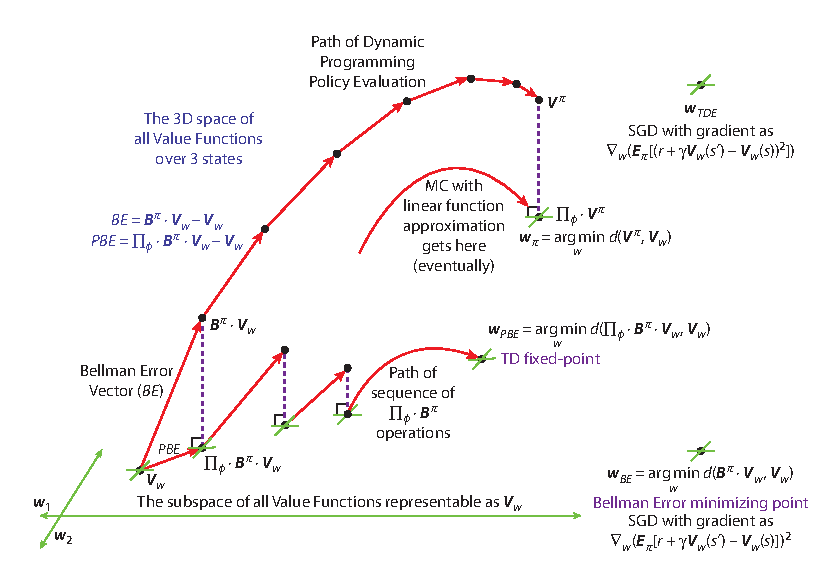
\includegraphics[scale=0.8]{vf_geometry.pdf}
\end{figure}
\end{frame}

\begin{frame}
\frametitle{Bellman Error (BE)-minimizing $\bm{w}_{BE}$}
\pause
$\bm{w}_{BE}$ is the vector in the $\bphi$ subspace for which the Bellman Error $\bb \cdot \vw - \vw$ is minimized
\begin{align*}
\bm{w}_{BE} & =  \argmin_{\bw} d(\bb \cdot \vw, \vw) \\
& = \argmin_{\bw} d(\vw, \brew + \gamma \bprob \cdot \vw) \\
& = \argmin_{\bw} d(\bphi \cdot \bw, \brew + \gamma \bprob \cdot \bphi \cdot \bw)\\
& = \argmin_{\bw} d(\bphi \cdot \bw - \gamma \bprob \cdot \bphi \cdot \bw, \brew)\\
& = \argmin_{\bw} d((\bphi - \gamma \bprob \cdot \bphi) \cdot \bw, \brew )\\
\end{align*}
\pause
This is a weighted least-squares linear regression of $\brew$ versus $\bphi - \gamma \bprob \cdot \bphi$
with weights $\bmu$, whose solution is:
\pause
$$\bm{w}_{BE} = ((\bphi - \gamma \bprob \cdot \bphi)^T \cdot \bd \cdot (\bphi - \gamma \bprob \cdot \bphi))^{-1} \cdot (\bphi - \gamma \bprob \cdot \bphi)^T \cdot \bd \cdot \brew$$
\end{frame}

\begin{frame}
\frametitle{Model-Free Learning of $\bm{w}_{BE}$}
\pause
\begin{itemize}[<+->]
\item Let us refer to $(\bphi - \gamma \bprob \cdot \bphi)^T \cdot \bd \cdot (\bphi - \gamma \bprob \cdot \bphi)$ as $\bm{A}$
\item Let us refer to $(\bphi - \gamma \bprob \cdot \bphi)^T \cdot \bd \cdot \brew$ as $\bm{b}$ 
\item So that $\bm{w}_{BE} = \bm{A}^{-1} \cdot \bm{b}$
\item Following policy $\pi$, each time we perform a model-free transition from $s$ to $s'$ getting reward $r$, we get a sample estimate of $\bm{A}$ and $\bm{b}$
\item Estimate of $\bm{A}$ is the outer-product of vector $\bm{\phi}(s) - \gamma \cdot \bm{\phi}(s')$ with itself
\item Estimate of $\bm{b}$ is scalar $r$ times vector $\bm{\phi}(s) - \gamma \cdot \bm{\phi}(s')$ 
\item Average these estimates across many such model-free transitions
\item However, this requires $m$ (number of features) to not be too large
\end{itemize}
\end{frame}


\begin{frame}
\frametitle{Residual Gradient Algorithm to solve for $\bm{w}_{BE}$}
\pause
\begin{itemize}[<+->]
\item $\bm{w}_{BE}$ is the vector in the $\bphi$ subspace for which BE is minimized
\item But BE for a state is the expected TD error $\delta$ in that state when following policy $\pi$
\item So we want to do SGD with gradient of square of expected TD error
\begin{align*}
\Delta \bw & = - \frac{1}{2} \alpha \cdot \nabla_{\bw} (\mathbb{E}_{\pi}[\delta])^2\\
& = - \alpha \cdot \mathbb{E}_{\pi}[r + \gamma \cdot \bm{\phi}(s')^T \cdot \bw - \bm{\phi}(s)^T \cdot \bw] \cdot \nabla_{\bw} \mathbb{E}_{\pi}[\delta]\\
& = \alpha \cdot (\mathbb{E}_{\pi}[r + \gamma \cdot \bm{\phi}(s')^T \cdot \bw] - \bm{\phi}(s)^T \cdot \bw) \cdot (\bm{\phi}(s) - \gamma \cdot \mathbb{E}_{\pi}[\bm{\phi}(s')])\\
\end{align*}
\item  This is called the {\em Residual Gradient} algorithm
\item Requires two independent samples of $s'$ transitioning from $s$
\item In that case, converges to $\bm{w}_{BE}$ robustly (even for non-linear approx)
\item But it is slow, and doesn't converge to a desirable place
\item Cannot learn if we can only access features, and not underlying states
\end{itemize}
\end{frame}


\begin{frame}
\frametitle{Temporal Difference Error (TDE)-minimizing $\bm{w}_{TDE}$}
\pause
\begin{itemize}[<+->]
\item $\bm{w}_{TDE}$ is the vector in the $\bphi$ subspace for which the expected square of the TD error $\delta$ (when following policy $\pi$) is minimized
$$\bm{w}_{TDE} = \argmin_{\bw} \sum_{s \in \mathcal{S}} \bmu(s) \sum_{r,s'} \mathbb{P}_{\pi}(r, s'|s) \cdot (r + \gamma \cdot \bm{\phi}(s')^T \cdot \bw - \bm{\phi}(s)^T \cdot \bw)^2$$
\item To perform SGD, we have to estimate the gradient of the expected square of TD error by sampling
\item The weight update for each sample in the SGD will be:
\begin{align*}
\Delta \bw & = - \frac{1}{2} \alpha \cdot \nabla_{\bw} (r + \gamma \cdot \bm{\phi}(s')^T \cdot \bw - \bm{\phi}(s)^T \cdot \bw)^2\\
& = \alpha \cdot (r + \gamma \cdot \bm{\phi}(s')^T \cdot \bw - \bm{\phi}(s)^T \cdot \bw) \cdot (\bm{\phi}(s) - \gamma \cdot \bm{\phi}(s'))\\
\end{align*}
\item This algorithm (named {\em Naive Residual Gradient}) converges robustly, but not to a desirable place
\end{itemize}
\end{frame}

\begin{frame}
\frametitle{Projected Bellman Error (PBE)-minimizing vector $\bm{w}_{PBE}$}
\pause
\begin{itemize}[<+->]
\item Consider the composition of Projection Operator $\bpi$ and Bellman Policy Operator $\bb$, i.e., $\bpi \cdot \bb$
\item We call $\bpi \cdot \bb$ the Projected Bellman Operator
\item Applying $\bb$ on a VF vector $\vw$ in the $\bphi$ subspace typically throws it out of the $\bphi$ subspace
\item Then further applying $\bpi$ brings it back into the $\bphi$ subspace
\item Call this resultant VF vector in the $\bphi$ subspace as $\bm{V_{w'}}$
\item Define $\bm{w}_{BE}$ as the $\bw$ for which $d(\bm{V_{w'}}, \vw)$ is minimized
\item Projected Bellman Error (PBE)-minimizing: $\bm{w}_{PBE} = \argmin_{\bw} d((\bpi \cdot \bb) \cdot \vw, \vw)$
\item The minimum is 0, i.e., $\bphi \cdot \bm{w}_{PBE}$ is the fixed point of $\bpi \cdot \bb$
\item Starting with an arbitrary VF vector $\bv$ and repeatedly applying $\bb$ (potentially taking it out of the subspace) followed by $\bpi$ (projecting it back to the subspace), we will reach the fixed point $\bphi \cdot \bm{w}_{PBE}$
\end{itemize}
\end{frame}


\begin{frame}
\frametitle{Solution of $\bm{w}_{PBE}$ with a Linear System Formulation}
\pause
$\bphi \cdot \bm{w}_{PBE}$ is the fixed point of operator $\bpi \cdot \bb$. We know:
$$\bpi = \bphi \cdot (\bphi^T \cdot \bd \cdot \bphi)^{-1} \cdot \bphi^T \cdot \bd$$
$$\bb (\bv) = \brew + \gamma \bprob \cdot \bv$$
\pause
Therefore,
$$\bphi \cdot (\bphi^T \cdot \bd \cdot \bphi)^{-1} \cdot \bphi^T \cdot \bd \cdot (\brew + \gamma \bprob \cdot \bphi \cdot \bm{w}_{PBE}) = \bphi \cdot \bm{w}_{PBE}$$
\pause
Since columns of $\bphi$ are assumed to be independent (full rank),
\begin{align*}
(\bphi^T \cdot \bd \cdot \bphi)^{-1} \cdot \bphi^T \cdot \bd \cdot (\brew + \gamma \bprob \cdot \bphi \cdot \bm{w}_{PBE}) & = \bm{w}_{PBE}\\
\bphi^T \cdot \bd \cdot (\brew + \gamma \bprob \cdot \bphi \cdot \bm{w}_{PBE}) &= \bphi^T \cdot \bd \cdot \bphi \cdot \bm{w}_{PBE}\\
\bphi^T \cdot \bd \cdot (\bphi - \gamma \bprob \cdot \bphi) \cdot \bm{w}_{PBE} &= \bphi^T \cdot \bd \cdot \brew\\ 
\end{align*}
\pause
This is a square linear system of the form $\bm{A} \cdot \bm{w}_{PBE} = \bm{b}$ whose solution is:
$$\bm{w}_{PBE} = \bm{A}^{-1} \cdot \bm{b} = (\bphi^T \cdot \bd \cdot (\bphi - \gamma \bprob \cdot \bphi))^{-1} \cdot \bphi^T \cdot \bd \cdot \brew$$
\end{frame}


\begin{frame}
\frametitle{Model-Free Learning of $\bm{w}_{PBE}$}
\pause
\begin{itemize}[<+->]
\item How do we construct matrix $\bm{A} = \bphi^T \cdot \bd \cdot (\bphi - \gamma \bprob \cdot \bphi)$ and vector $\bm{b} = \bphi^T \cdot \bd \cdot \brew$ without a model?
\item Following policy $\pi$, each time we perform a model-free transition from $s$ to $s'$ getting reward $r$, we get a sample estimate of $\bm{A}$ and $\bm{b}$
\item Estimate of $\bm{A}$ is outer-product of vectors $\bm{\phi}(s)$ and $\bm{\phi}(s) - \gamma \cdot \bm{\phi}(s')$
\item Estimate of $\bm{b}$ is scalar $r$ times vector $\bm{\phi}(s)$ 
\item Average these estimates across many such model-free transitions
\item This algorithm is called Least Squares Temporal Difference (LSTD)
\item Alternative: Our usual Semi-Gradient TD descent with updates:
$$\Delta \bw = \alpha \cdot (r + \gamma \cdot \bm{\phi}(s')^T \cdot \bw - \bm{\phi}(s)^T \cdot \bw) \cdot \bm{\phi}(s)$$
\item This converges to $\bm{w}_{PBE}$ because $\mathbb{E}_{\pi}[\Delta \bw] = 0$ yields
$$ \bphi^T \cdot \bd \cdot (\brew + \gamma \bprob \cdot \bphi \cdot \bw - \bphi \cdot \bw) = 0$$
$$ \Rightarrow \bphi^T \cdot \bd \cdot (\bphi - \gamma \bprob \cdot \bphi) \cdot \bw = \bphi^T \cdot \bd \cdot \brew$$ 
\end{itemize}
\end{frame}


\begin{frame}
\frametitle{Gradient TD Algorithms to solve for $\bm{w}_{PBE}$}
\pause
\begin{itemize}[<+->]
\item For on-policy linear func approx, semi-gradient TD works
\item For non-linear func approx or off-policy, we need Gradient TD
\begin{itemize}
\item GTD: The original Gradient TD algorithm
\item GTD-2: Second-generation GTD
\item TDC: TD with Gradient correction
\end{itemize}
\item We need to set up the loss function whose gradient will drive SGD
$$\bm{w}_{PBE} = \argmin_{\bw} d(\bpi \cdot \bb \cdot \vw, \vw) = \argmin_{\bw} d(\bpi \cdot \bb \cdot \vw, \bpi \cdot \vw)$$
\item So we define the loss function (denoting $\bb \cdot \vw - \vw$ as $\bdel$) as:
$$\mathcal{L}({\bf w})  = (\bpi \cdot \bdel)^T \cdot \bd \cdot (\bpi \cdot \bdel) = \bdel^T \cdot \bpi^T \cdot \bd \cdot \bpi \cdot \bdel$$
$$=  \bdel^T \cdot (\bphi \cdot (\bphi^T \cdot \bd \cdot \bphi)^{-1} \cdot \bphi^T \cdot \bd)^T \cdot \bd \cdot  (\bphi \cdot (\bphi^T \cdot \bd \cdot \bphi)^{-1} \cdot \bphi^T \cdot \bd) \cdot \bdel$$
$$= \bdel^T \cdot (\bd \cdot \bphi \cdot (\bphi^T \cdot \bd \cdot \bphi)^{-1} \cdot \bphi^T) \cdot \bd \cdot  (\bphi \cdot (\bphi^T \cdot \bd \cdot \bphi)^{-1} \cdot \bphi^T \cdot \bd) \cdot \bdel$$
$$= (\bdel^T \cdot \bd \cdot \bphi) \cdot (\bphi^T \cdot \bd \cdot \bphi)^{-1} \cdot (\bphi^T \cdot \bd \cdot  \bphi) \cdot (\bphi^T \cdot \bd \cdot \bphi)^{-1} \cdot (\bphi^T \cdot \bd \cdot \bdel)$$
$$= (\bphi^T \cdot \bd \cdot \bdel)^T \cdot (\bphi^T \cdot \bd \cdot \bphi)^{-1} \cdot (\bphi^T \cdot \bd \cdot \bdel)$$
\end{itemize}
\end{frame}

\begin{frame}
\frametitle{TDC Algorithm to solve for $\bm{w}_{PBE}$}
\pause
We derive the TDC Algorithm based on $\nabla_{\bw} \mathcal{L}({\bw})$
$$\nabla_{\bw} \mathcal{L}({\bw}) = 2 \cdot (\nabla_{\bw} (\bphi^T \cdot \bd \cdot \bdel)^T) \cdot (\bphi^T \cdot \bd \cdot \bphi)^{-1} \cdot (\bphi^T \cdot \bd \cdot \bdel)$$
\pause
Now we express each of these 3 terms as expectations of model-free transitions $s \stackrel{\pi}\longrightarrow (r,s')$, denoting $r + \gamma \cdot \bm{\phi}(s')^T \cdot \bw - \bm{\phi}(s)^T \cdot \bw$ as $\delta$
\pause
\begin{itemize}[<+->]
\item $\bphi^T \cdot \bd \cdot \bdel = \mathbb{E}[\delta \cdot \bm{\phi}(s)]$
\item $\nabla_{\bw} (\bphi^T \cdot \bd \cdot \bdel)^T = \mathbb{E}[(\nabla_{\bw} \delta) \cdot \bm{\phi}(s)^T] = \mathbb{E}[(\gamma \cdot \bm{\phi}(s') - \bm{\phi}(s)) \cdot \bm{\phi}(s)^T]$
\item $\bphi^T \cdot \bd \cdot \bphi = \mathbb{E}[\bm{\phi}(s) \cdot \bm{\phi}(s)^T]$
\end{itemize}
\pause
Substituting, we get:
$$\nabla_{\bw} \mathcal{L}({\bw}) = 2 \cdot  \mathbb{E}[(\gamma \cdot \bm{\phi}(s') - \bm{\phi}(s)) \cdot \bm{\phi}(s)^T] \cdot \mathbb{E}[\bm{\phi}(s) \cdot \bm{\phi}(s)^T]^{-1} \cdot \mathbb{E}[\delta \cdot \bm{\phi}(s)]$$
\end{frame}

\begin{frame}
\frametitle{Weight Updates of TDC Algorithm}
\pause
$$\Delta \bw  = - \frac {1} {2} \alpha \cdot \nabla_{\bw} \mathcal{L}({\bw})$$
$$ = \alpha \cdot \mathbb{E}[(\bm{\phi}(s) - \gamma \cdot \bm{\phi}(s')) \cdot \bm{\phi}(s)^T] \cdot \mathbb{E}[\bm{\phi}(s) \cdot \bm{\phi}(s)^T]^{-1} \cdot \mathbb{E}[\delta \cdot \bm{\phi}(s)]$$
$$ = \alpha \cdot (\mathbb{E}[\bm{\phi}(s) \cdot \bm{\phi}(s)^T] - \gamma \cdot \mathbb{E}[\bm{\phi}(s') \cdot \bm{\phi}(s)^T]) \cdot \mathbb{E}[\bm{\phi}(s) \cdot \bm{\phi}(s)^T]^{-1} \cdot \mathbb{E}[\delta \cdot \bm{\phi}(s)]$$
$$ = \alpha \cdot (\mathbb{E}[\delta \cdot \bm{\phi}(s)] - \gamma \cdot \mathbb{E}[\bm{\phi}(s') \cdot \bm{\phi}(s)^T] \cdot \mathbb{E}[\bm{\phi}(s) \cdot \bm{\phi}(s)^T]^{-1} \cdot \mathbb{E}[\delta \cdot \bm{\phi}(s)])$$
$$ = \alpha \cdot (\mathbb{E}[\delta \cdot \bm{\phi}(s)] - \gamma \cdot \mathbb{E}[\bm{\phi}(s') \cdot \bm{\phi}(s)^T] \cdot \btheta)$$
\pause
\vspace*{2mm}

$\btheta = \mathbb{E}[\bm{\phi}(s) \cdot \bm{\phi}(s)^T]^{-1} \cdot \mathbb{E}[\delta \cdot \bm{\phi}(s)]$ is the solution to weighted least-squares linear regression of $\bb \cdot \bv - \bv$ against $\bphi$, with weights as $\mu_{\pi}$.
\pause
\vspace*{3mm}

{\bf Cascade Learning: Update both $\bw$ and $\btheta$} ($\btheta$ converging faster)
\pause
\begin{itemize}[<+->]
\item $\Delta \bw = \alpha \cdot \delta \cdot \bm{\phi}(s)  - \alpha \cdot \gamma \cdot \bm{\phi}(s') \cdot (\btheta^T \cdot \bm{\phi}(s))$
\item $\Delta \btheta = \beta \cdot (\delta - \btheta^T \cdot \bm{\phi}(s)) \cdot \bm{\phi}(s)$
\end{itemize}
\pause
Note: $\btheta^T \cdot \bm{\phi}(s)$ operates as estimate of TD error $\delta$ for current state $s$
\end{frame}

\begin{frame}
\frametitle{Key Takeaways from this Chapter}
\pause
\begin{itemize}[<+->]
\item Batch RL makes efficient use of data
\item DQN uses Experience-Replay and fixed Q-learning targets, avoiding the pitfalls of time-correlation and semi-gradient
\item LSTD is a direct (gradient-free) solution of Batch TD Prediction
\item LSPI is an off-policy, experience-replay Control Algorithm using LSTDQ for Policy Evaluation
\item Optimal Exercise of American Options can be tackled with LSPI and Deep Q-Learning algorithms
\item Value Function Geometry provides tremendous intuition
\item Projected Bellman Error (PBE) is the right loss function to use
\item The gradient of PBE loss function yields Gradient TD algorithms
\end{itemize}
\end{frame}


\end{document}
